\documentclass[12pt]{article}

\usepackage{ucs} 
\usepackage[utf8x]{inputenc} % Включаем поддержку UTF8  
\usepackage[russian]{babel}  % Включаем пакет для поддержки русского языка  
\usepackage{graphicx}
\usepackage{hyperref}

%\definecolor{linkcolor}{HTML}{799B03} % цвет ссылок
%\definecolor{urlcolor}{HTML}{799B03} % цвет гиперссылок
%\hypersetup{pdfstartview=FitH,  linkcolor=linkcolor,urlcolor=urlcolor, colorlinks=true}

\begin{document}
Моим заданием является воссоздание математической модели по части кода.
\newline
В формуле для расчёта площади многоугольника, взятого из репозитория: 
[ \href{https://github.com/EAZYBOT/Python/blob/master/lab1/l3.py}{1} ]
(строчки 52-58)
\begin{figure}[h]
\center{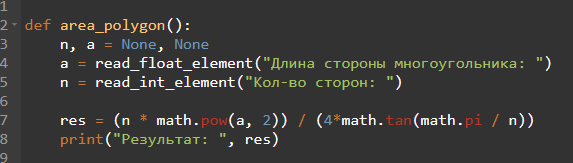
\includegraphics[width=1\linewidth]{Cap1.png} \\Код программы}
\end{figure}

Это формула для вычисления площади многоугольника
\newline
Тут считаем, что многоугольник правильный и все его стороны одинаковые.
Площадь многоугольника S мы ищем через формулу:
\begin{eqnarray} 
    S &=& \frac{na^{2}}{4\tan({\frac{\Big{\pi}}{\Big{n}})}} 
  \end{eqnarray} 
\begin{description}
\center{Формула расчёта площади многоугольника}
\end{description}
где n - это кол-во сторон многоугольника;
\par
a - длина сторон.
\\

[1] Python\textunderscore lab1\textunderscore l3.py at master · EAZYBOT\textunderscore Python · GitHub : [сайт]. – Сан-Франциско, 2008 – . – URL: \newline
https://github.com/EAZYBOT/Python/blob/master/lab1/l3.py (дата обращения: 22.09.2023). – Текст : электронный.
\end{document}	